\documentclass{article}
\usepackage{enumitem}


\usepackage{rotating}


\usepackage{listings}
\begin{document}

\begin{figure}[t]
\centering
	
\includegraphics[height=6.25cm,keepaspectratio]{Figures/logo}
\end{figure}

\title{TrackMe \\ Software Engineering 2 Project\\ \textit{ATD Document} }
\author{Stefano Martina, Alessandro Nichelini, Francesco Peressini
		\\ \\ A.Y. 2018/2019 \\ Version 1.1.0}
		
\maketitle
\newpage

\tableofcontents
\newpage

\section{Introduction}

\subsection{Purpose and Scope} 
The Acceptance Test Document has the purpose of evaluating the adherence of the implementation with respect to the  documents previously delivered.\newline
To do so, we have considered the three documents available in the provided repository.

\subsection{Reference} 
	As said above, we used the three documents, as referenced below:
	\begin{itemize}
		\item RASD Document : Requirements Analysis and Specification Document
		\begin{itemize}			\item v1.2 - 12/01/2019		\end{itemize}	
		\item DD Document : Design Document
		\begin{itemize}			\item v1.1 - 12/01/2019		\end{itemize}	
		\item ITD Document: Implementation and Testing Document
		\begin{itemize}			\item v1.0 - 13/01/2019		\end{itemize}	
	\end{itemize}
\subsection{Overview} 

\section{Project}
\subsection{Project info}


\newpage
\section{Installation Setup}
\subsection{Backend }
\subsubsection{Installation and launch}
	We have installed the backend as explained in the ITD Document, with the only exception of the particular system dependent command (we tested it on macOS).\newline
	We have installed the following module with \textit{"brew"} command:
	\begin{itemize}
		\item \textbf{PostgreSQL} an open source object-relational database system
		\begin{itemize}
			\item	installed with the command : \textit{brew install postgresql}
		\end{itemize}
		\item \textbf{NodeJS} an asynchronous event driven JavaScript runtime
		\begin{itemize}
			\item	installed with the command : \textit{brew install nodejs}
		\end{itemize}
	\end{itemize}
	After the launch of the postgres service with the command : \textit{brew services start postgresql}, we create a new database and a new role for the admin user. \newline
	Then, with the new role just created we import the dump of the database provided in the Implementation folder of the previously mentioned repository.
	As last step we have configured the \textit{"start.sh"} file with the following configuration and we launched it with the command \textit{"node app.js"}.
	\begin{figure}[h!]
		\centering
		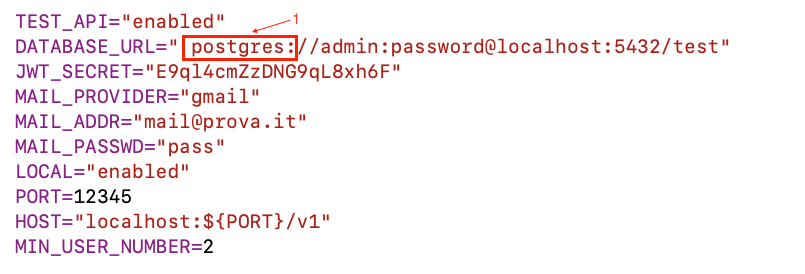
\includegraphics[height=4.25cm,keepaspectratio]{Figures/error1}
	\end{figure}
	
\subsubsection{Conslusion}
We didn't encounter particular issues, the guide lines are clear and enough explicative.\newline
The only thing which makes sense to be mentioned is one error encountered during the database connection. It always responds with "message: role //password// does not exists". This is due to a small error in the configuration file, probably due to the fact that is a machine dependant parameter (view image 1).

\newpage	
\subsection{Frontend}
\subsubsection{Installation and launch}
Regarding the mobile application we have installed the provided APK file on an Android Smartphone. We also tried to install it on a few simulators.\newline
Regarding the web app, we launched it using the command \textit{"python3 -m http.server"}, as explained into the guide lines a.
\subsubsection{Conclusion}
Following the instruction on the ITD Document, on a smartphone, everything works correctly.
Doing the same steps on a simulator the application crashes, probably due to some incompatibilities with the running version on the simulator.	\newline
The web-app launch works correctly.
\newpage



\section{Acceptance Test}
\subsection{Tests}
We are going to test the implementation of each requirements that has been implemented according to ITD document provided.

\subsubsection{Actor registration}
\begin{itemize}
	\item [RM$_M$]: \textit{OK.} Users actually can register providing information required, but registration process succeed also without an associated smartwatch.
	\item [R2$_M$]: \textit{OK.} Implementation works: registration process is successfull if and only there is not another user with the same email/fiscal code. However error handling is not able to distinguish between a duplicate email or fiscal code.
	\item [R11$_M$]: \textit{OK.} Organizers can successfully resister.
	\item [R1$_W$]: \textit{OK.} Companies can successfully register.
	\item [R14$_C$]: \textit{OK.} Information such as birthday and fiscal code are validated trough UI form.
\end{itemize}

\subsection{Actor Authentication}
\begin{itemize}
	\item [R1$_M$]: \textit{OK.} Users can successfully log in in the application.
	\item [R12$_M$]: \textit{OK.} Organisers can successfully log in in the application.
	\item [R2$_W$]: \textit{OK.} Companies  can successfully log in in the application.
\end{itemize}

\subsection{Individuals Management}
\begin{itemize}
	\item [R6$_M$]: \textit{OK.} Requests appear in the right section of the mobile app. Users can effectively accept or decline them.
	\item [R2$_C$]: \textit{OK.} Users received notification about new request at the email address used during 
	\item registration.
\end{itemize}

\subsection{Data management}
\begin{itemize}
	\item [R4$_C$]: \textit{OK.} We can't directly test this feature, but it seems that all data loaded to the application are available after a logout, then it has been probably implemented right.
	\item [R5$_C$]: \textit{OK.} Same of the previously one.
	\item [R2$_S$]: ??????.
\end{itemize}

\subsection{Query management}
\begin{itemize}
	\item [R6$_W$]: \textit{UNKNOWN.} See section issues.
	\item [R7$_W$]: \textit{OK.} Companies can actually request data of individuals. 
	\item [R8$_W$]: \textit{OK.} Companies can access to individuals data trough the web site.
	\item [R9$_W$]: \textit{OK.} The website actually provides data download capabilities.
	\item [R6$_C$]: \textit{OK.}
	\item R6bisW: \textit{OK.} The website gives capability of subscribe trough a slider. The company actually receives a notification when a new data is available.
	\item R7C: \textit{KO.} Check in issues section

\subsubsection{Issues}

For what regards the implementation of requirements R6W, we were not able to check if the queries work because the system kept telling us that the parameters inserted were too restrictive.\\

During the testing of requirements R7W, R8W, we have found the following issue:
\begin{itemize}
	\item the process fails if requests are made by a company that has the same email address of a user. The error message is the following: \textit{"Error: Unauthorized. Retry"} and it appears on the website as an alert. However, since it's unlikely that a company uses the same address of a users, we still marked the requirements as "OK".
\end{itemize}

\subsection{Race management}
\begin{itemize}
	\item [R8$_M$]: \textit{OK.} Registration is possibile trough the track4run tab at anytime.
	\item [R9$_M$]: \textit{KO.} Check in issues section.
	\item [R13$_M$]: \textit{OK.} Organisers actually have all the needed to create a path.
	\item [R14$_M$]: \textit{OK.} Organisers actually have all the needed to define run informations and path.
\end{itemize}

\subsubsection{issues}
For what concerning requirements R9M: application only displays the name of the run, its status and the position of participants. Information about the starting point, the ending point, the precise path, the run length are not available.

\subsection{Users Spectating Race}
\begin{itemize}
	\item [R10$_M$]: \textit{OK.} Participants position are correctly displayed.
	\item [R13$_C$]: ????????
\end{itemize}


\subsection{Issue}
\subsubsection{Issue1}
\subsubsection{Issue2}
\subsubsection{Issue3}


\subsection{Revision history}
\begin{itemize}
	\item 1.0.0 - Initial version (11/11/2018)

\end{itemize}
\subsection{Document Structure}

\newpage










\newpage
\section{Effort spent}

\begin{itemize}
	\item Stefano Martina: 35.00h
	\item Alessandro Nichelini: 37.00h
	\item Francesco Peressini: 37.00h
\end{itemize}

\end{document}